\documentclass[conference, onecolumn]{IEEEtran} % Replace onecolumn with twocolumn if needed
% Report template for Mälardalen University
% Original template can be found: 
% https://www.overleaf.com/latex/templates/ieee-bare-demo-template-for-conferences/ypypvwjmvtdf
% Template file structure organised by: Emil Persson
% The following packages should follow the IEEE conference guidelines.

% Swedish language package 
\usepackage[utf8]{inputenc}
\usepackage[T1]{fontenc}
\usepackage[swedish,english]{babel}

% Graphics
\usepackage{graphicx, float, subfigure, blindtext}

\newcommand\IEEEhyperrefsetup{
bookmarks=true,bookmarksnumbered=true,%
colorlinks=true,linkcolor={black},citecolor={black},urlcolor={black}%
}

% Preferred hyperref setup, Michael Shell
\usepackage[\IEEEhyperrefsetup, pdftex]{hyperref}

% Maths
\usepackage{mathtools}

% These packages must be at the end
\usepackage[nolist,nohyperlinks]{acronym}
\usepackage{cleveref}
\graphicspath{{images/}}
% \acrodef{acronym}[short name]{full name}
\acrodef{IC}[IC]{Integrated Circuit}
% \acrodef{svm}[SVM]{Support Vector Machine}
\newacro{svm}[SVM]{Support Vector Machine}
% Example use \ac{IC} for printing "Integrated Circuit (IC), use \ac{IC} again and it will print (IC)"
% For plural use \acp{IC} for short and \aclp{IC} for long.
% For more see: http://ftp.acc.umu.se/mirror/CTAN/macros/latex/contrib/acronym/acronym.pdf

% Swedish language package 
\usepackage[utf8]{inputenc}
\usepackage[T1]{fontenc}
\usepackage[swedish,english]{babel}

% Graphics
\usepackage{graphicx, float, subfigure, blindtext}

% \newcommand\IEEEhyperrefsetup{
% bookmarks=true,bookmarksnumbered=true,%
% colorlinks=true,linkcolor={black},citecolor={black},urlcolor={black}%
% }

% Preferred hyperref setup, Michael Shell
% \usepackage[\IEEEhyperrefsetup, pdftex]{hyperref}

% Maths
\usepackage{mathtools}
\usepackage{multirow}
% These packages must be at the end
\usepackage[nolist,nohyperlinks]{acronym}
\usepackage{cleveref}
\graphicspath{{images/}}

% Remove section first paragraph indent
\usepackage{titlesec}
\titlespacing*{\section}{0pt}{*1}{*1}
\titlespacing*{\subsection}{0pt}{*1}{*1}
\renewcommand{\thesubsubsection}{\arabic{subsubsection}}
\titleformat{\subsubsection}[runin]{\itshape}{\thesubsubsection)}{1em}{}[:]
\titlespacing*{\subsubsection}{\parindent}{0pt}{*1}

% Include authors
\author{\IEEEauthorblockN{
Carl-Johan Höglind\IEEEauthorrefmark{1},
Author 2\IEEEauthorrefmark{2}
}

\IEEEauthorblockA{
School of Innovation, Design and Engineering\\
Mälardalen University, Västerås, Sweden\\
Email:
\IEEEauthorrefmark{1}chd16002@student.mdu.se,
\IEEEauthorrefmark{2}author2@student.mdu.se
}}

% The report title.
\title{Assignment 2, Embedded Systems II\\
Mälardalen University}

% Document begins here
\begin{document}

    % Create the title.
    \maketitle
    % Example sections, name them according to specific needs.
    \section{Question 1} 

    \section{Question 2}
        \subsection{a}
            Sufficient schedulability test for RM scheduling: $U <= n(2^{1/n} - 1)$ \\ where n is the number of tasks in the task set and U is the processor utilization factor, $U = \sum_{i=1}^{n} \frac{C_i}{T_i}$. 

        \renewcommand{\arraystretch}{1.4}
        \begin{figure}[H]
        \centering
        \begin{minipage}{0.5\textwidth}
            \begin{table}[H]
            \centering
            \begin{tabular}{|l|l|l|}
                \hline
                \textbf{Task}   & \textbf{T=D}  & \textbf{C}  \\ \hline
                A               & 3             & 1           \\ \hline
                B               & 5             & 2           \\ \hline
                C               & 2             & 0.5         \\ \hline

            \end{tabular}
            \end{table}
        \end{minipage}%
        \caption{Task set}
        \label{fig:Taskset}
        \end{figure}
    \renewcommand{\arraystretch}{1.0}

        \subsubsection{Task set schedulable?}
        $U = \sum_{i=1}^{n} \frac{C_i}{T_i} = \frac{1}{3} + \frac{2}{5} + \frac{0.5}{2} = 0.98$ \\
        $U <= n(2^{1/n} - 1) = 3(2^{1/3} - 1) = 0.78$ \\
        Since the statement $U <= n(2^{1/n} - 1)$ is false in this case, the task set cannot be proven to be schedulable with this sufficient test method.

        \subsection{b}
            \subsubsection{Exact schedulability test, Tracing}
            \begin{figure}[H]
                \centering
                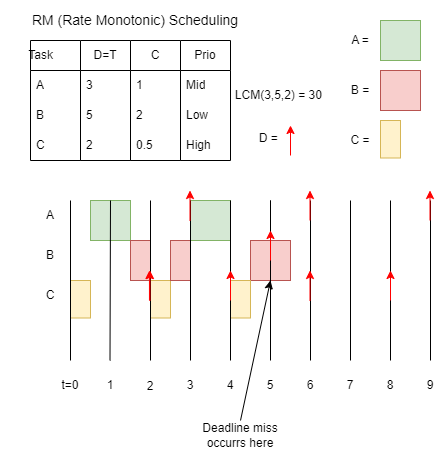
\includegraphics[width=0.5\textwidth]{images/Ass1Q2.drawio.png}
                \caption{Tracing of the task set proves that it is not schedulable with RM.}
                \label{fig:tracing}
            \end{figure}

            As demonstrated in figure \ref{fig:Taskset}, the task set is not schedulable with RM scheduling. The task set is not schedulable because task B misses its deadline at $t = 5$.

    % Select the IEEEtran style
    %\bibliographystyle{IEEEtran}
    % Include bibliography file
    %\bibliography{IEEEabrv, refs}

\end{document}